\documentclass[a4paper, 12pt]{article}
%pack{{{
\usepackage[utf8]{inputenc}
\usepackage[russian]{babel}
\usepackage{pdfpages}
%}}}
\begin{document}
\section*{Netbench}
Инструмент позволяет измерить пропускную способность канала между двумя хостами, 
имитировать нагрузку на сеть.

Набор состоит их следующих инструментов:
\begin{itemize}
	\item Модуль сервера приложения тестирования пр. способности
	\item Модуль клиента приложения тестирования пр. способности
	\item Модуль имитации нагрузки на сеть
\end{itemize}

\subsection*{Приложение-сервер}
Может устанавливать соединения с несколькими приложениями-клиентами.
Порт по умолчанию 3333. Есть возможность изменить его. 
Возможно ограничить количество клиентов.
\subsection*{Приложение-клиент}
Для функционирования неоходимо установить соединение с сервером.
Сразу после удачного подключения начинает отображаться текущая скорость соединения.
\subsection*{Имитатор нагрузки}
Генерация большого количества UDP-пакетов и посылка их по указанному адресу.
\newpage
%\subsection*{Предполагаемая схема использования}
%\nonewpage
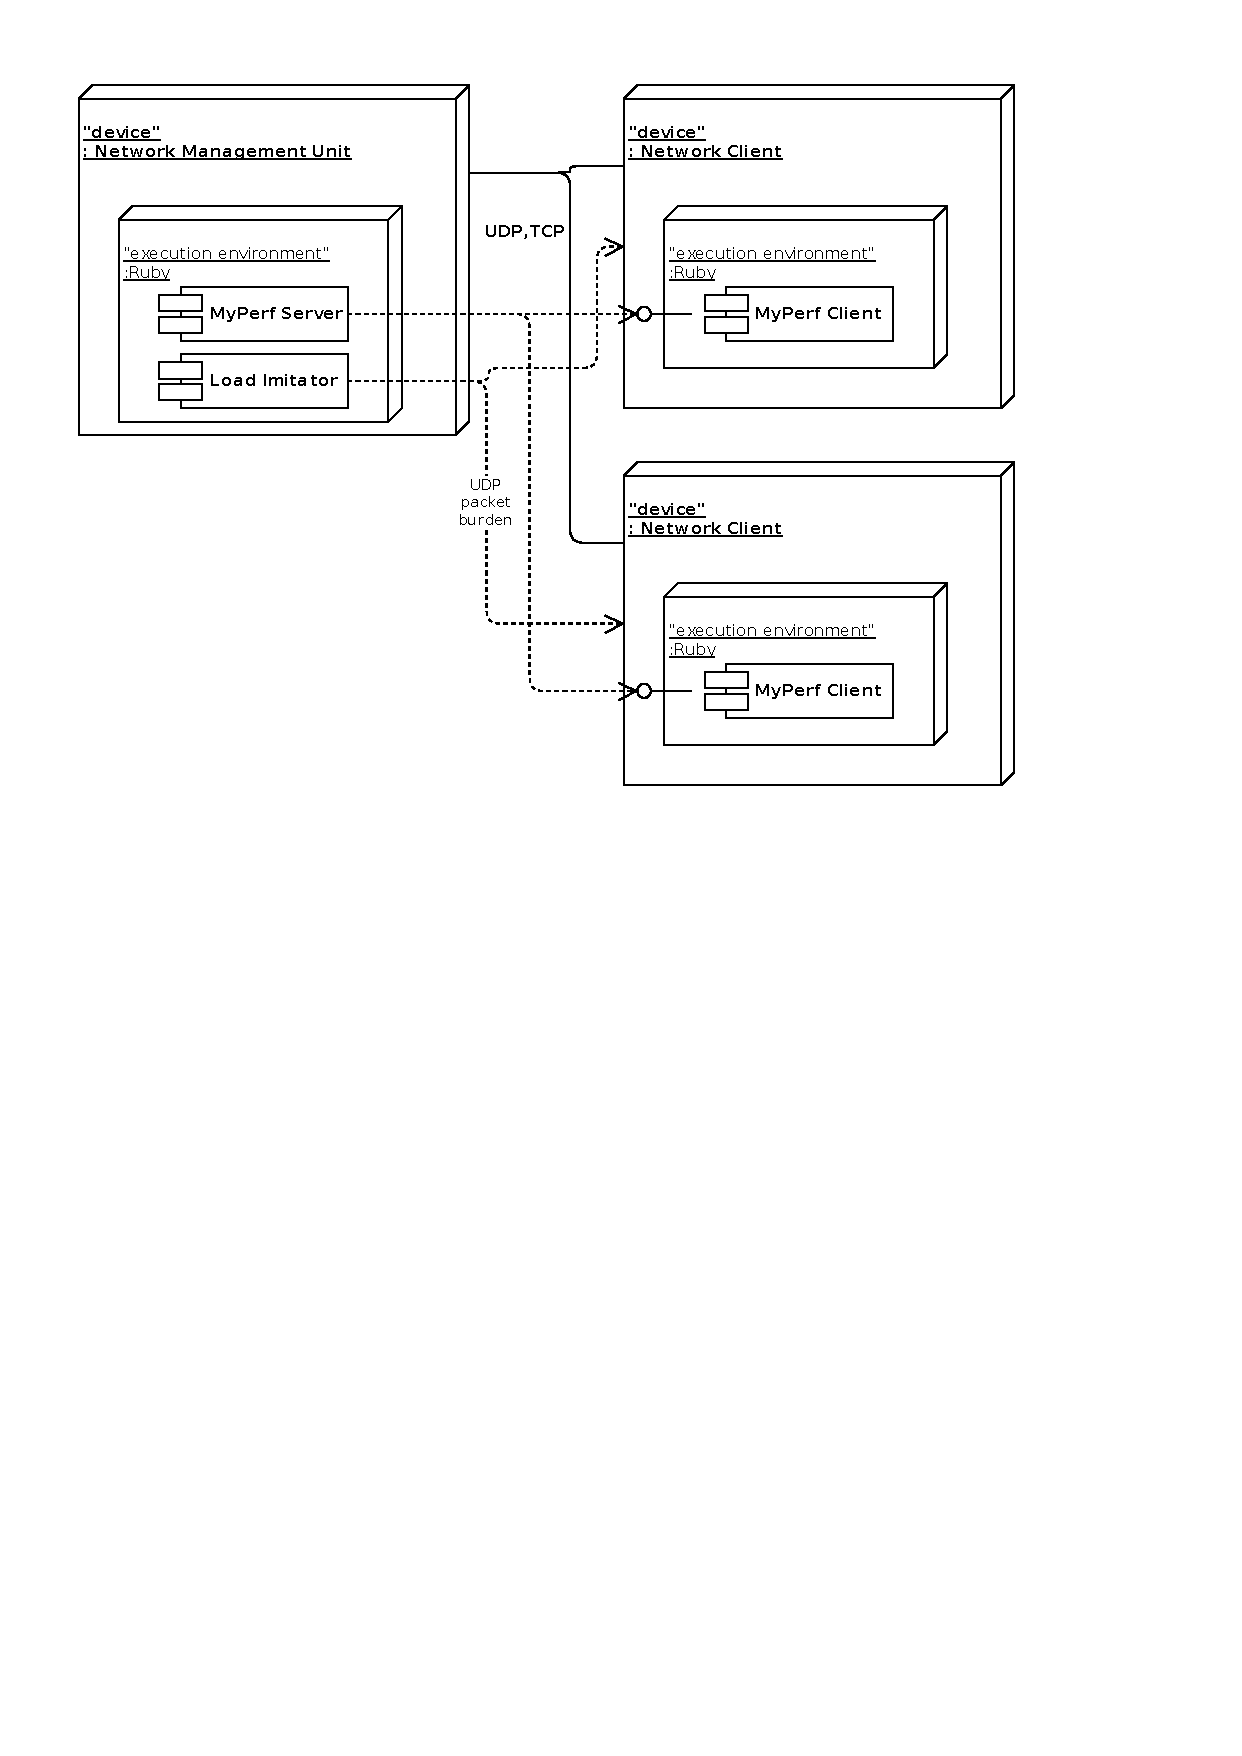
\includepdf[pages=1,pagecommand=\section*{Предполагаемая схема использования},offset=0 -5cm]{ndia.pdf}
%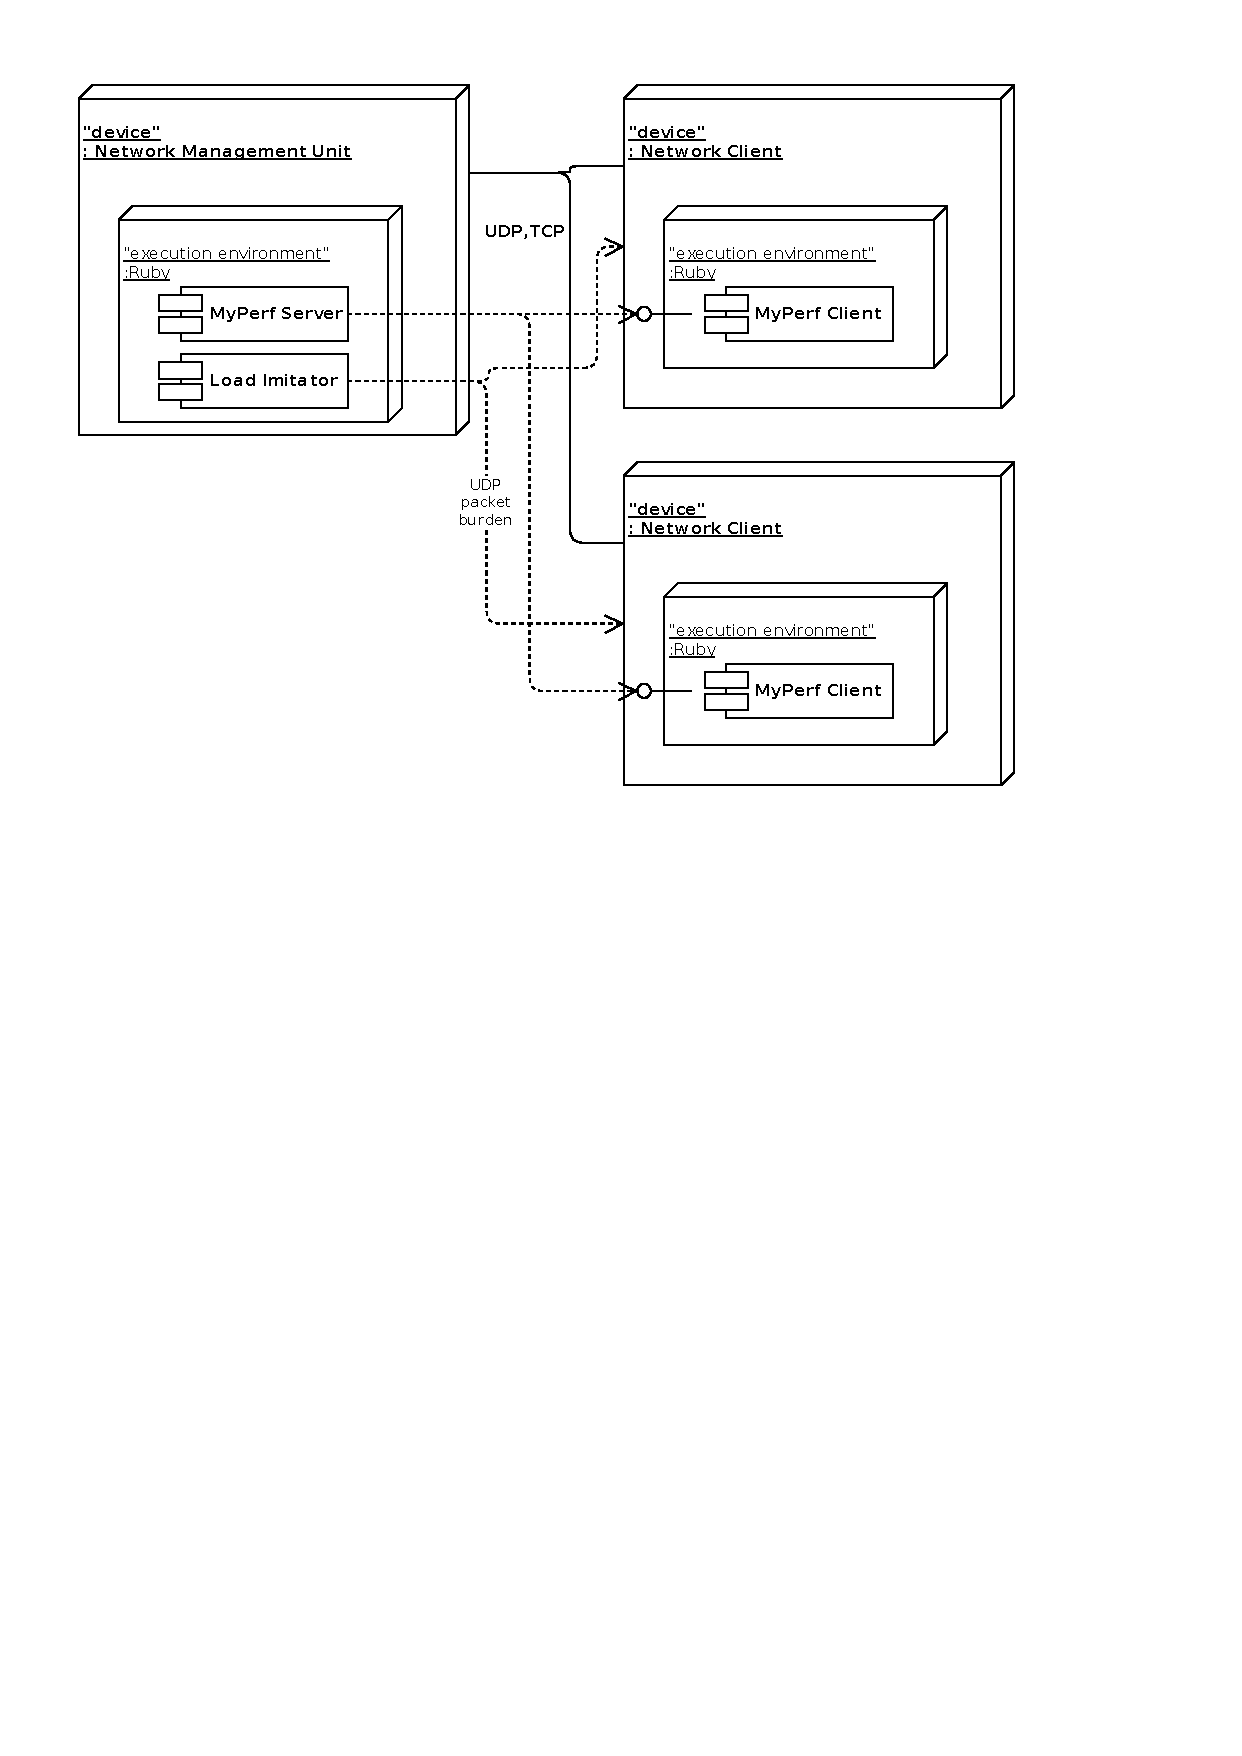
\includepdf[pages={-}]{ndia.pdf}
%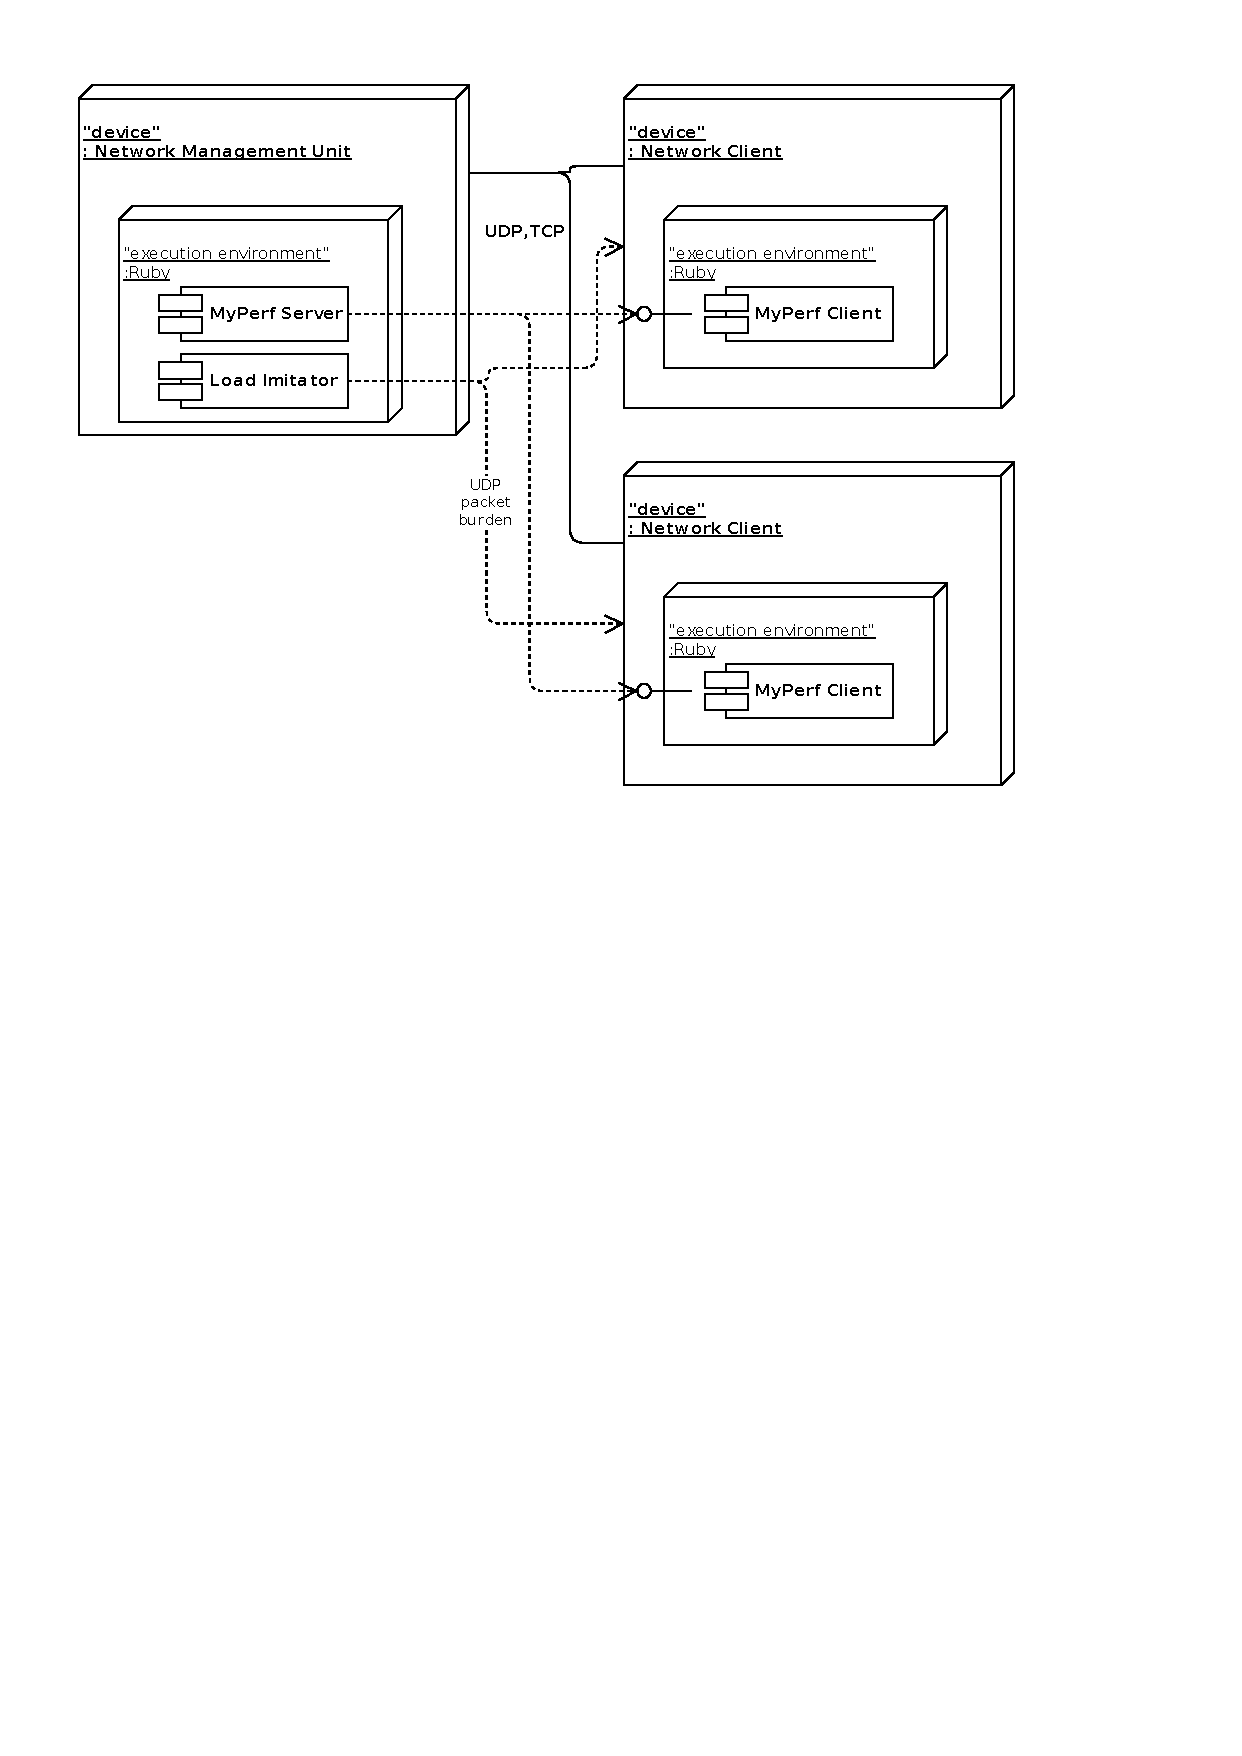
\includegraphics{ndia.pdf}
\end{document}
